\documentclass[conference]{IEEEtran}

\usepackage[utf8]{inputenc}

\PassOptionsToPackage{bookmarks=false}{hyperref}

\usepackage{amsmath}
\usepackage{float}

\usepackage{listings}
\usepackage{color}
\usepackage{graphicx}
\usepackage{tikz}
\usepackage[caption=true,font=footnotesize]{subfig}
\usepackage[hidelinks]{hyperref}

\graphicspath{ gfx/ }

\definecolor{lbcolor}{rgb}{0.9,0.9,0.9}
\definecolor{dkgreen}{rgb}{0,0.6,0}
\definecolor{gray}{rgb}{0.5,0.5,0.5}
\definecolor{mauve}{rgb}{0.58,0,0.82}

\newcommand*\circled[1]{\tikz[baseline=(char.base)]{
		\node[shape=circle,draw,inner sep=1pt] (char) {#1};}}

\lstset{
  basicstyle=\normalsize ,
  backgroundcolor=\color{lbcolor},
  %frame=tb,
  language=C++,
  aboveskip=6mm,
  belowskip=3mm,
  numbers=left,
  showstringspaces=false,
  columns=flexible,
  basicstyle={\small\ttfamily},
  numbers=none,
  numberstyle=\tiny\color{gray},
  keywordstyle=\color{blue},
  commentstyle=\color{dkgreen},
  stringstyle=\color{mauve},
  breaklines=true,
  breakatwhitespace=true,
  captionpos=b,
  tabsize=3
}

% Additional new commands
\newcommand{\etal}{{\em et al. }}
\newcommand{\cL}{{\cal L}}
\newcommand{\map}{\texttt{map} }
\newcommand{\unmap}{\texttt{unmap} }
\newcommand{\rb}{\texttt{readBuffer} }
\newcommand{\rsec}[1]{Section~\ref{sec:#1}}
\newcommand{\rsecs}[2]{Sections~\ref{sec:#1} --~\ref{sec:#2}}
\newcommand{\rtab}[1]{Table~\ref{tab:#1}}
\newcommand{\rfig}[1]{Figure~\ref{fig:#1}}
\newcommand{\rfigs}[2]{Figures~\ref{fig:#1} --~\ref{fig:#2}}
\newcommand{\rlst}[1]{Listing~\ref{lst:#1}}
\newcommand{\rfign}[3]{Figures~\ref{fig:#1}, \ref{fig:#2} \& \ref{fig:#3}}
\newcommand{\rlsts}[2]{Listings~\ref{lst:#1}~--~\ref{lst:#2}}
\newcommand{\rlstn}[3]{Listings~\ref{lst:#1}{#2}~--~\ref{lst:#1}{#3}}
\newcommand{\req}[1]{Equation~\ref{eq:#1}}
\newcommand{\reqs}[2]{Equations~\ref{eq:#1} --~\ref{eq:#2}}
\newcommand{\ttt}[1]{{\texttt{#1}}}
\newcommand{\tit}[1]{{\textit{#1}}}
\newcommand{\citex}[1]{\cite{XX}\ }

\newenvironment{filecode}[1][]
{\minipage{0.9\linewidth}% \begin{filecode}[#1]
	\lstset{basicstyle=\ttfamily\footnotesize,frame=single,float=ht,#1}}
{\endminipage}% \end{filecode}

\IEEEoverridecommandlockouts
% The preceding line is only needed to identify funding in the first footnote. If that is unneeded, please comment it out.
\usepackage[portuguese, english]{babel}
\usepackage{amsmath,amssymb,amsfonts}
\usepackage{algorithmic}
\usepackage{textcomp}
\def\BibTeX{{\rm B\kern-.05em{\sc i\kern-.025em b}\kern-.08em
    T\kern-.1667em\lower.7ex\hbox{E}\kern-.125emX}}
\begin{document}

\title{Estudos em Regressão Linear}

\author{\IEEEauthorblockN{Matheus Mortatti Diamantino}
\IEEEauthorblockA{
RA 156740 \\
matheusmortatti@gmail.com}
\and
\IEEEauthorblockN{Jos\'{e} Renato Vicente}
\IEEEauthorblockA{
RA 155984\\
joserenatovi@gmail.com}}

\maketitle

\section{Introdução}

Este projeto teve como intuito o estudo prático do método de regressão linear em Machine Learning. Foram utilizado os algoritmos de \textit{Gradient Descent} conhecidos como \textit{Stochastic, Batch, Mini Batch e Equação Normal}, de modo a compara-los em termos de complexidade e acurácia.~\cite{sandra}

Foi feito um estudo de predição de preço de diamantes, utilizando uma base de dados com 54000 exemplos, em que são apresentados seus preços e nove features como tamanho, cor e número de quilates.

\section{Atividades}

\subsection{Regressão Linear}

Regressão Linear é um método muito conhecido de Machine Learning, utilizado para predizer o valor de uma variável dependente baseado em valores de variáveis independentes. Essa regressão é chamada linear porque se considera que a relação da resposta às variáveis é uma função linear de alguns parâmetros. Desta forma, dado um vetor Theta de tamanho igual ao número de features, cujo valor queremos determinar, temos que:

\begin{equation} \label{eq:hx}
PreçoAlvoEsperado = \sum_{i=1}^{m} \theta_{i}X_{i} = h_{\theta}(x)
\end{equation}

Em que X é um vetor com os valores das features para um dado diamante, cujo preço queremos determinar.Para encontrar esse valor de Theta, utilizaremos alguns algoritmos e compararemos os resultados obtidos com cada um.

Cada algoritmo utilizado é baseado no método de \textit{Descrida de Gradiente (ou Gradient Descent)}. Este é um método utilizado para achar o ponto mínimo de uma função, aproximando gradativamente seu valor até um ponto quando não é possível ser diminuido mais (i.e. a derivada da função neste ponto é zero). Este método consegue apenas achar mínimos locais e, com isso, não é garantido que o resultado obtido é o melhor para o dado problema.

Para medirmos a eficácia do algoritmo, utilizamos uma \textit{Função de Custo} que nos diz o quão perto do resultado desejado estamos, dado um conjunto de dados. Esta função é definida por:

\begin{equation} \label{eq:cost_function}
J(\theta) = \dfrac{1}{2m} \sum_{i=1}^{m}(h_{\theta}(x^{i}) - y^{i})^2
\end{equation}

Como queremos minimizar a função de custo, queremos que cada passo da nossa descida de gradiente se aproxime mais do mínimo local. Para extrairmos a direção que temos que ir, utilizamos a derivada da função de custo:

\begin{equation} \label{eq:cost_derivative}
\dfrac{\partial J}{\partial \theta_{j}} = \dfrac{1}{m} \sum_{i=1}^{m}(h_{\theta}(x^{i}) - y^{i}) x^{i}
\end{equation}

Logo, para aproximarmos os valores de $\theta$ de modo a nos aproximar do mínimo local, utilizamos a fórmula

\begin{equation} \label{eq:gradient_descent}
\theta_{j} := \theta_{j} - \alpha \dfrac{1}{m} \sum_{i=1}^{m}(h_{\theta}(x^{i}) - y^{i}) x^{i}
\end{equation}

, onde $0 \leq j \leq m$, $x_{0} = 1$ e $\alpha$ é o que chamamos de \textit{Learning Rate} que define o quão agressivamente tentaremos nos aproximar do mínimo. Este método de descida de gradiente é chamada de \textit{Batch Gradient Descent}. A seguir, veremos três outras variações deste algoritmo

\paragraph{Stochastic Gradient Descent}

Neste método, utiliza-se apenas um exemplo de treino para cada passo da descida de gradiente. Deste modo, a equação~\ref{eq:gradient_descent} se transforma em

\begin{equation} \label{eq:stochastic_descent}
\theta_{j} := \theta_{j} - \alpha(h_{\theta}(x^{i}) - y^{i}) x^{i}
\end{equation}

Utiliza-se este método quando procura-se rapidez de execução. Contudo, um ponto negativo deste método é que, como usamos como amostra apenas um exemplo de treino, um passo pode nos levar a um custo mais alto. Como o número de iterações é alta, porém, o método converge ao mínimo e mais eficientemente do que o \textit{Batch} até um certo limite.

\paragraph{Mini Batch Gradient Descent}

Para obtermos um resultado balanceado, utiliza-se uma mistura dos métodos \textit{Batch} e \textit{Stochastic}, em que define-se um tamanho para o lote de exemplos de treino que serão utilizados para atualizar cara $\theta$.

\begin{equation} \label{eq:minibatch_descent}
\theta_{j} := \theta_{j} - \alpha \dfrac{1}{m} \sum_{i=k}^{k+b-1}(h_{\theta}(x^{i}) - y^{i}) x^{i}
\end{equation}

, onde $b$ é o tamanho do lote, $k = 0, b, 2b, ..., m-1$.

\paragraph{Equação Normal}

Para a regressão linear, é possível derivar uma fórmula direta para o ponto de mínimo local que desejamos. Para isso, utilizamos manipulações matriciais na forma~\cite{ayearofai}

\begin{equation} \label{eq:normal}
\theta = (X^{T}X)^{-1}X^{T}y
\end{equation}

, onde $X$ é a matriz de features, $y$ é a matriz dos dados que queremos prever e $\theta$ é a matriz dos coeficientes de $h(X)$.

\subsection{Normalização de Features}

Como cada feature tem seu valor em uma escala diferente (i.e. algumas estão na ordem de milhares e outras na ordem de centenas), o processo de descida do gradiente poderá acontecer de forma lenta. Isso se dá pelo fato de que a atualização dos $\theta$s não ocorrerá de forma uniforme entre as features, já que a distância de um dado $\theta_{i}$ a seu valor esperado pode ser maior do que de outro $\theta_{j}, j \neq i$. Assim, realizamos o que é chamado de \textit{Normalização de Features}, onde colocamos todas as features $x_{i}$ em um valor entre $ \-0.5 \leq x_{i} \leq 0.5$. Isso é feito através da fórmula:

\begin{equation} \label{eq:feature_norm}
x_{i} = \dfrac{x_{i} - \dfrac{size(x_{i})}{2}}{size(x_{i})}
\end{equation}

\subsection{Transformação de Features}

Em alguns casos, podemos ter features que não possuem um valor no domínio dos números reais. Por exemplo, uma feature pode representar a cor de um dado elemento. Deste modo, é necessário realizar uma transformação de tais features para o domínio dos reais. Para realizar tal transformação, criamos uma nova feature para cada possível valor da feature que queremos transformar, de modo que, se para o exemplo de dado $e_{i}$ temos que esta feature possui um valor $x_{j}$, a nova feature correspondente a $x_{j}$ terá o valor $1$ e as demais features criadas terão o valor $0$. Tomemos como exemplo uma feature de Cor que pode receber os valores \textit{Azul, Amarelo, Vermelho e Verde}. Assim, o resultado da transformação acontecerá da seguinte forma:

\begin{table}[H]
\centering
\begin{tabular}{|c|c|c|c|c|}
\hline
Feature $x_{i}$ & Azul & Amarelo & Vermelho & Verde \\ \hline
Azul            & 1    & 0       & 0        & 0     \\ \hline
Amarelo         & 0    & 1       & 0        & 0     \\ \hline
Vermelho        & 0    & 0       & 1        & 0     \\ \hline
Verde           & 0    & 0       & 0        & 1     \\ \hline
\end{tabular}
\end{table}

Onde cada coluna representa a nova feature criada e cada linha representa o valor original da feature $x_{i}$.

\subsection{Regularização}

Regularização é um método utilizado para \textit{evitar} overfitting dos dados. É relizado de forma a penalizar os valores de $\theta$ para que estes mantenham valores pequenos, sendo menos propenso ao overfitting. Isto é feito na forma de um novo parâmetro $\lambda$ que definirá o quanto cada $\theta$ será penalizado:

\begin{equation} \label{eq:regularization}
\theta_{j} := \theta_{j} * (1 - \lambda * \dfrac{\alpha}{m}) - \alpha \dfrac{1}{m} \sum_{i=1}^{m}(h_{\theta}(x^{i}) - y^{i}) x^{i}
\end{equation}

Este valor deve ser modificado de forma a melhorar o resultado final. Se o valor for muito alto, a influência da regularização pode ser negativa, criando um aumento no erro final. Se muito baixo, não terá o efeito desejado. Vale mencionar que a regularização na equação normal se da pela forma

\begin{equation} \label{eq:normal_reg}
\theta = (X^{T}X + \lambda I)^{-1}X^{T}y
\end{equation}

, onde $I$ é a matriz identidade.

\subsection{Base de Dados}

Foi utilizado uma base de dados sobre Diamantes, a qual descreve diferentes aspectos sobre o diamante como cor, claridade e quilate, e apresenta seu preço. O objetivo deste projeto foi de utilizado o método de \textit{Regressão Linear} descrito acima para prever o preço de um dado diamante, dado suas características.

\section{Soluções Propostas}

\subsection{Tratamento dos Dados}

Para obtermos melhores resultados, começamos por realizar o tratamento dos dados. Para isso, foram aplicados os métodos de \textit{Normalização} descritos na seção anterior. Também, foi aplicado uma \textit{Transformação de Features} nas features \textit{Cut, Color e Clarity}, pois seus valores são descritos por uma string.

\subsection{Algoritmos Implementados}

Com o objetivo de compara-los, foram implementados os algoritmos \textit{Batch, Mini Batch, Stochastic e Equação Normal} como solução para a Regressão Linear.

\paragraph{Algoritmos Iterativos}

Algoritmos iterativos para a \textit{Descida de Gradiente} precisam de um critério de parada para sua execução. Tais critérios foram, demonstrados pela Listagem~\ref{lst:criterio_parada}:

\begin{itemize}
  \item Número máximo de iterações.
  \item Valor máximo da a diferença entre os $\theta$s originais e novos.
\end{itemize}

\begin{filecode}[label=lst:criterio_parada,caption=Criterios de Parada para os algoritmos de Descida do Gradiente]
  \lstset{numbers=left}
	\lstinputlisting[language=Python]{gfx/criterio_parada.py}
\end{filecode}

Foi implementado também uma solução para o caso onde a função de custo diverge devido a um $\alpha$ muito alto. Caso o custo corrente seja maior do que o último custo calculado, o valor de $\alpha$ é diminuido por um fator pré definido, de modo que a descida aconteça com menores riscos de divergência, como demonstrado pela Listagen~\ref{lst:learning_rate_change}.

\begin{filecode}[label=lst:learning_rate_change,caption=Modo como o fator $\alpha$ é modificado]
  \lstset{numbers=left}
	\lstinputlisting[language=Python]{gfx/learning_rate_change.py}
\end{filecode}

\paragraph{Regularização}

Para todas as soluções implementadas, foi utilizado o método de regularização para melhorar os resultados e evitar \textit{Overfitting}. Foi seguido os métodos descritos acima para a implementação tanto na forma da \textit{Equação Normal} quanto para os algoritmos iterativos.

\section{Experimentos e Discussão}

Os experimentos foram realizados em uma máquina que possui um processador Intel Core i7-6700HQ com 4 cores rodando a 2.60GHz e 16GB de RAM, com Ubuntu 16.04.

\begin{figure*}[h]
	\centering
	\subfloat[Stochastic with $\lambda$ = 0.0000005, $\alpha$ = 0.01]{
		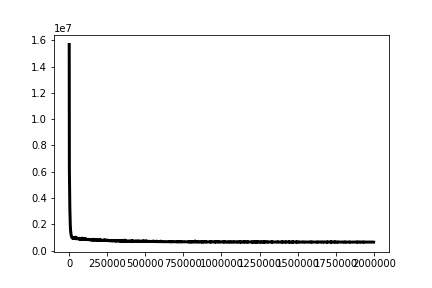
\includegraphics[width=0.5\linewidth]{gfx/S_costitr_mitr2000000.png}
		\label{fig:sto_5m}
	}

  \subfloat[Mini Batch with $\lambda$ = 0.0000005, $\alpha$ = 0.01]{
		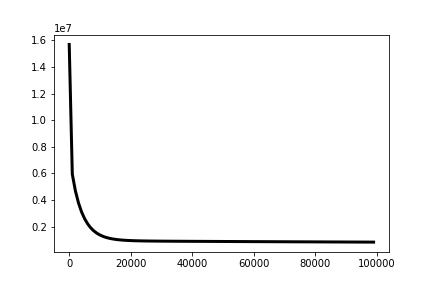
\includegraphics[width=0.5\linewidth]{gfx/MB_costitr_mitr100000_b1000.png}
		\label{fig:mb_1m}
	}
  \caption{Gráficos de Custo x Iterações para cada algoritmo}
	\label{fig:results}
\end{figure*}



\section{Conclusions and Future Work}

The main conclusions of the work as well as some future directions for other people interested in continuing this work.

\bibliographystyle{IEEEtran}
\bibliography{biblio-link,biblio}

\end{document}
